\chapter{Research Methodology}\label{ch:methodology}

This chapter outlines the methodology used to develop \cs{}, a document retrieval system (DRS) tailored for Mindanao State University -- Iligan Institute of Technology (MSU-IIT). It is adapted from Pallavi Sinha's framework for building LLM-powered applications \citep{sinha2024}, shown in Figure~\ref{fig:sinha}. The framework has eight steps; this study follows the first six, from use case discovery to the development of the application, and leaves out observability and deployment pipelines, which fall outside the project's development window. The structured approach ensures that \cs{} meets MSU-IIT's specific needs, following best practices in AI development such as iterative testing, ethical considerations, and data-driven refinement \citep{amershi2019}. Sections~\ref{sec:use-case} to~\ref{sec:development} follow the six adopted phases in order, and Section~\ref{sec:evaluation-procedure} describes how the system is evaluated.

\begin{figure}[htbp]
  \centering
  % Sinha's eight steps for building LLM-powered applications; steps 1-6 were adopted.
\begin{tikzpicture}[
    phase/.style={accent=3.1cm, minimum height=1.55cm},
    skipped/.style={muted=3.1cm, minimum height=1.55cm, text=ink!60},
    num/.style={circle, draw=maroon, fill=white, font=\footnotesize\bfseries, text=maroon, inner sep=1.5pt, minimum size=5mm},
    numskip/.style={num, draw=line, text=ink!50},
    node distance=0.55cm and 0.55cm]
  \node[phase] (s1) {\textbf{Use case discovery}\\[1pt]\footnotesize a feasible problem an LLM can solve};
  \node[phase, right=of s1] (s2) {\textbf{Prototype building}\\[1pt]\footnotesize a simple app around a pre-trained LLM};
  \node[phase, right=of s2] (s3) {\textbf{LLM system strategy}\\[1pt]\footnotesize single LLM, agent or multi-agent};
  \node[phase, right=of s3] (s4) {\textbf{LLM setup}\\[1pt]\footnotesize choose models by cost, latency, accuracy};
  \node[phase, below=1.1cm of s4] (s5) {\textbf{LLM hosting}\\[1pt]\footnotesize local servers or cloud};
  \node[phase, left=of s5] (s6) {\textbf{Development}\\[1pt]\footnotesize the application, with testing};
  \node[skipped, left=of s6] (s7) {\textbf{Observability}\\[1pt]\footnotesize logging, monitoring, alerts};
  \node[skipped, left=of s7] (s8) {\textbf{Deployment}\\[1pt]\footnotesize CI/CD and hosting of the app};
  \foreach \i in {1,...,6} \node[num] at (s\i.north west) {\i};
  \foreach \i in {7,8} \node[numskip] at (s\i.north west) {\i};
  \draw[arrow] (s1) -- (s2);
  \draw[arrow] (s2) -- (s3);
  \draw[arrow] (s3) -- (s4);
  \draw[arrow] (s4) -- (s5);
  \draw[arrow] (s5) -- (s6);
  \draw[arrow, draw=line] (s6) -- (s7);
  \draw[arrow, draw=line] (s7) -- (s8);
  \node[note, anchor=north] at ($(s7.south)!0.5!(s8.south)+(0,-0.15)$) {not part of the study's six phases};
\end{tikzpicture}

  \caption{Steps for Building LLM-Powered Applications, Adapted from \citet{sinha2024}; Steps 1--6 Were Adopted}\label{fig:sinha}
\end{figure}

\section{Use Case Discovery}\label{sec:use-case}

The proponents observed that MSU-IIT's current document retrieval system posed challenges for students, faculty, and staff. The keyword-based search often failed to return relevant results when queries didn't match exact terms, making it difficult to find necessary documents. For instance, searching for ``policy updates'' might miss files labeled differently, such as ``revised regulations.'' These limitations revealed the system's lack of contextual understanding and highlighted the need for a more intelligent solution. \cs{} addresses this by integrating OCR, vector similarity search, and LLM-based chat interfaces, enabling semantic search and conversational interaction to improve search accuracy and user experience.

\subsection{Process of Document Collection and Preparation}\label{sec:collection}

Building on the identified limitations of MSU-IIT's traditional document retrieval system, the study moves toward developing and evaluating a more intelligent solution. To ensure that the system is tested under realistic and representative conditions, the process begins with the careful collection and preparation of institutional documents. These documents are sourced from two main repositories: (1)~MSU-IIT's internal document archive, IIT Docs \citep{msuiitdocs}, and (2)~the MSU System Board of Regents (BOR) Resolutions archive \citep{msuiitbor}.

Both scanned and text-based PDF files are gathered, curated, and pre-processed to serve as the dataset for evaluating the proposed DRS. This step ensures the inclusion of a wide variety of document types, formats, and complexities, particularly those that require Optical Character Recognition (OCR) for interpretation. To maintain relevance and comprehensiveness, specific criteria were observed in selecting the documents:

\begin{itemize}
  \item \textbf{Relevance:} files were chosen based on their alignment with commonly referenced administrative functions and institutional topics.
  \item \textbf{Diversity of content:} the dataset includes policies, designations, incentives, travel orders, suspensions, and Charter Day issuances.
  \item \textbf{Format variety:} both scanned and digitally produced PDFs were included to assess the system's handling of OCR and different file structures.
  \item \textbf{Structural complexity:} documents with tables, multiple sections, watermarks, and typewritten text were included to test the retrieval capabilities rigorously.
\end{itemize}

Table~\ref{tab:corpus} summarizes the resulting corpus of 50 PDF files: five per category and repository, 25 from each repository. Two files are byte-for-byte duplicates of other files and are recognized as such on upload, leaving 48 distinct documents with 158 pages, issued between 1970 and 2024. Thirteen files have no text layer at all (pure scans), and most of the others carry a text layer produced by the repositories' own OCR, of varying quality; 33 of the 48 documents are a single page long, and the longest has 36 pages.

\begin{table}[htbp]
  \centering
  \caption{Composition of the Document Corpus}\label{tab:corpus}
  \begin{tabular}{@{}lccc@{}}
    \toprule
    \textbf{Category} & \textbf{IIT Docs} & \textbf{BOR Resolutions} & \textbf{Total} \\
    \midrule
    Charter Day   & 5 & -- & 5 \\
    Designation   & 5 & 5  & 10 \\
    Incentive     & 5 & 5  & 10 \\
    Policy        & 5 & 5  & 10 \\
    Suspension    & -- & 5 & 5 \\
    Travel Order  & 5 & 5  & 10 \\
    \midrule
    \textbf{Total} & \textbf{25} & \textbf{25} & \textbf{50} \\
    \bottomrule
  \end{tabular}
\end{table}

This comprehensive document preparation process sets the foundation for a meaningful evaluation of \cs{}'s ability to overcome the limitations of the current system and deliver more accurate, context-aware search results.

\subsection{Problem Definition and Stakeholders}

The development of \cs{} was motivated by critical limitations observed in the existing DRS at MSU-IIT. The institution relies on two primary repositories: the BOR Resolutions Archive, which governs MSU System policies, and IIT Docs, a repository of Special Orders, Memorandum Orders, and administrative issuances built on Google Drive's keyword-based search. While functional, these systems exhibit significant shortcomings:

\begin{enumerate}
  \item \textbf{Semantic blindness.} The keyword-only mechanism fails to interpret contextual nuances or semantic relationships, leading to irrelevant or incomplete results. Queries for ``Special Orders'' miss documents labeled with abbreviations like ``SO''; synonym-rich content (``academic calendar'' versus ``term schedule'') remains undiscovered; and paraphrased queries (``student allowances'' versus ``financial aid'') yield inconsistent results.
  \item \textbf{Format exclusion.} Scanned or image-based PDFs are excluded from search results because the repositories lack OCR. Documents with complex layouts, such as tables, multi-column text, or handwritten annotations, are similarly unsearchable.
  \item \textbf{Rigid interaction.} Users cannot refine queries iteratively because there is no conversational interface, which forces them to rely on repetitive keyword adjustments.
\end{enumerate}

The primary stakeholders are \textbf{students}, who need timely access to academic policies (for example, scholarship resolutions and enrollment guidelines) and event announcements, and \textbf{staff}, who locate memoranda (for example, procurement procedures and compliance records) to streamline operational workflows.

\section{Agent Prototype Building}\label{sec:prototype}

The first prototype was built between January and April 2025 to validate the idea before full development. It used a Django REST API, a React interface, Marker for OCR, LangChain's recursive text splitter, a pgvector store, and models running locally in Ollama. Several local models were compared on sample MSU-IIT documents for text generation, question answering, and semantic similarity search, considering response accuracy, latency, and resource use (Table~\ref{tab:prototype-models}).

\begin{table}[htbp]
  \centering
  \caption{Local Models Compared During Prototype Building (January--April 2025)}\label{tab:prototype-models}
  \small
  \begin{tabularx}{\linewidth}{@{}lX@{}}
    \toprule
    \textbf{Model (Ollama)} & \textbf{Observation} \\
    \midrule
    \multicolumn{2}{@{}l}{\emph{Language models}} \\
    \code{llama3.1:8b} & Strong language understanding, but too demanding for real-time use on the available hardware. \\
    \code{llama3.2:1b} & Light, but insufficient for conversations that need deep contextual understanding. \\
    \code{qwen3:1.7b} & Good language ability, but struggled with long documents. \\
    \code{qwen2.5:7b-instruct-q4\_K\_M} & Followed instructions well, with higher latency. \\
    \code{llama3.1:8b-text-fp16} & Good text processing at a higher resource cost. \\
    \code{llama3.1:8b} (4-bit) & Selected for the prototype: the best balance of quality and resource use \citep{metaai2024}. \\
    \midrule
    \multicolumn{2}{@{}l}{\emph{Embedding models}} \\
    \code{bge-m3} & Multilingual, but in this prototype weaker on names, numbers and local terms. \\
    \code{mxbai-embed-large} & Selected for the prototype for its precision on such entities (1024 dimensions) \citep{mixedbread2024}. \\
    \bottomrule
  \end{tabularx}
\end{table}

The prototype established three lessons that shaped the final design. First, on CPU-only hardware even the selected 8-billion-parameter model answered slowly, and OCR of a scanned page took longer still, so model hosting had to be separated from the application (Section~\ref{sec:hosting}). Second, dense embeddings alone missed exact identifiers such as reference numbers and surnames, whichever embedding model was used; the final system therefore pairs BGE-M3 with a keyword index and fuses the two (Section~\ref{sec:rrf}), which recovers exactly the queries on which BGE-M3 had looked weaker. Third, answers needed visible evidence to be trusted, which led to numbered, page-level citations.

\section{LLM System Strategy}\label{sec:strategy}

Strategic design decisions were made on model selection, embedding strategy, and document chunking. \cs{} uses a \emph{single agent with one tool}: one language model reads the question and the conversation, decides whether and what to search, calls the search tool up to three times per question, and writes the answer from the passages it retrieved. This was preferred over a multi-agent design, which suits complex tasks that need several specialized roles \citep{chen2023}; answering from a document library needs one well-grounded retrieval loop, and a single agent is simpler to build, faster, and easier to evaluate. Document processing, by contrast, is a fixed pipeline rather than an agent (Section~\ref{sec:algorithms}), because every document goes through the same steps.

All language models are used zero-shot (Section~\ref{sec:zero-shot}). Every model in the system is \emph{open-weight}: its weights are published under a license that allows the institution to download and run it on its own hardware. Because the proponents have no GPU server of their own, the models are reached through OpenRouter, a service that hosts the same open models behind one API; the system can be moved to self-hosted copies of the same weights without changing its behavior (Section~\ref{sec:hosting}). Table~\ref{tab:models} lists the models and their roles.

\begin{table}[htbp]
  \centering
  \caption{Open-Weight Models Used by \cs{}}\label{tab:models}
  \small
  \begin{tabularx}{\linewidth}{@{}>{\raggedright\arraybackslash}p{3.6cm}>{\raggedright\arraybackslash}p{2.0cm}X@{}}
    \toprule
    \textbf{Model} & \textbf{License} & \textbf{Role in \cs{}} \\
    \midrule
    Surya OCR 2 (0.69B) & OpenRAIL & Marker's OCR engine: reads the text of every page, run locally with llama.cpp. \\
    Qwen3-VL-30B-A3B-Instruct & Apache-2.0 & Marker's LLM mode (tables, forms, handwriting), cataloguing, chat answers, chat titles. \\
    BGE-M3 (0.57B) & MIT & Embeddings of passages and queries (1024 dimensions, multilingual). \\
    Qwen3-Reranker-8B & Apache-2.0 & Reranking of the fused search results. \\
    \bottomrule
  \end{tabularx}
\end{table}

\section{LLM Setup}\label{sec:llm-setup}

One of the key processes of this study is choosing the right LLM setup. This section explains how a language model works and why each model in Table~\ref{tab:models} was chosen.

\subsection{LLM Underlying Process}

According to \citet{mulugeta2023}, a Large Language Model operates through a series of structured processes to interpret and generate human-like text, illustrated in Figure~\ref{fig:llm-process}. The prompt is split into tokens (Section~\ref{sec:tokens}), each token is mapped to a vector that also encodes its position, and a stack of transformer layers relates every token to every other through self-attention \citep{vaswani2017}. The final layer yields a probability for every possible next token; the decoder picks one (at temperature 0, the most likely; at higher temperatures, with some randomness), appends it, and repeats until it produces a stop token. Training, which builds these weights, falls outside the scope of this study: \cs{} uses pre-trained models as they are.

\begin{figure}[htbp]
  \centering
  % How an LLM turns a prompt into text, one token at a time (after Mulugeta, 2023).
\begin{tikzpicture}[
    st/.style={accent=2.25cm, minimum height=1.25cm},
    io/.style={muted=1.9cm, minimum height=1.25cm, text=ink},
    node distance=0.42cm]
  \node[io] (in) {\textbf{Prompt}\\\footnotesize text};
  \node[st, right=of in] (tok) {\textbf{Tokenizer}\\\footnotesize text $\to$ token IDs};
  \node[st, right=of tok] (emb) {\textbf{Embedding}\\\footnotesize IDs $\to$ vectors + positions};
  \node[st, right=of emb] (tr) {\textbf{Transformer}\\\footnotesize self-attention layers};
  \node[st, right=of tr] (dec) {\textbf{Decoding}\\\footnotesize next-token probabilities};
  \node[io, below=1.0cm of dec] (out) {\textbf{Output}\\\footnotesize text};
  \foreach \a/\b in {in/tok, tok/emb, emb/tr, tr/dec, dec/out} \draw[arrow] (\a) -- (\b);
  \coordinate (l1) at ($(dec.south west)+(0.35,0)$);
  \coordinate (l2) at ($(emb.south east)+(-0.35,0)$);
  \draw[arrow] (l1) -- ++(0,-0.55) -| node[note, pos=0.25, below] {append the chosen token, repeat} (l2);
\end{tikzpicture}

  \caption{How a Large Language Model Generates Text, After \citet{mulugeta2023}}\label{fig:llm-process}
\end{figure}

\subsection{Marker and Surya OCR 2}

Marker converts PDF files to Markdown \citep{marker2025}. Version 2 performs OCR with Surya OCR 2, a 0.69-billion-parameter vision-language model trained to transcribe document images, which it serves through llama.cpp, an efficient inference engine for open models \citep{surya2025,llamacpp2025}. Marker first detects the text lines and layout blocks of each page, then has Surya OCR 2 read every block, ignoring any existing text layer, and finally assembles the blocks into Markdown in reading order. Marker was the OCR tool of the defended prototype; version 2 replaces its earlier recognition models with this vision-language model.

\paragraph{LLM mode.} Marker can additionally send the regions it finds hardest---tables, forms, handwriting, and complex regions---to a general vision-language model, which corrects their text using the image \citep{marker2025}. \cs{} enables this mode with Qwen3-VL-30B-A3B-Instruct. The combination keeps the strength of each model: Surya OCR 2 transcribes characters faithfully, including unusual surnames that a general model may ``normalize'', while Qwen3-VL restructures the tables of stipend rates and incentive amounts that line-by-line OCR tends to flatten. Section~\ref{sec:converter-comparison} compares this setup with Docling, MarkItDown, and the vision model on its own.

\subsection{Qwen3-VL-30B-A3B-Instruct}

Qwen3-VL-30B-A3B-Instruct is an open-weight vision-language model released under the Apache-2.0 license \citep{qwen3vl2025}. It is a \emph{mixture-of-experts} model: of its roughly 31 billion parameters, only about 3 billion are active for each token, so it answers about as fast as a 3-billion-parameter model while drawing on the knowledge of a much larger one. It accepts page images, follows instructions in many languages including Filipino, calls tools, and produces output that conforms to a JSON schema, which covers every language task in \cs{}: Marker's LLM mode, cataloguing, chat answers, and chat titles. Using one model for all four keeps self-hosting simple, since only one large model has to be served.

\subsection{BGE-M3}

BGE-M3 is a multilingual text-embedding model of 0.57 billion parameters released under the MIT license \citep{chen2024bgem3}. It maps passages of up to 8,192 tokens to 1024-dimensional vectors and supports over 100 languages, so questions in Filipino or Cebuano can still find English passages. It is small enough to run on a CPU.

\subsection{Qwen3-Reranker-8B}

A reranker, or cross-encoder, reads the query and a candidate passage \emph{together} and outputs a relevance score \citep{nogueira2019}. This is more accurate than comparing two independently computed embeddings, but too slow to apply to the whole library, so \cs{} applies it only to the 20 best candidates after rank fusion. Qwen3-Reranker-8B is released under the Apache-2.0 license \citep{qwen3reranker2025}.

\subsection{Local Configuration with Ollama}\label{sec:local-mode}

For confidential records that must not leave the campus network, as required by the Data Privacy Act of 2012 \citep{dpa2012}, \cs{} can run every model locally through Ollama, an open-source runtime for language models \citep{ollama2024}. In this configuration the answers and catalogue come from Qwen3-4B-Instruct (4-bit), chat titles from Qwen3-1.7B, embeddings from BGE-M3, OCR from Marker with Surya OCR 2, and Marker's LLM mode from a local vision model such as Qwen3-VL-8B. The switch is a single setting; the pipeline, search, and agent are unchanged. Because the smaller local models have an 8,192-token context window, long documents take the map-reduce path of Algorithm~\ref{alg:summary} (Section~\ref{sec:mapreduce-theory}).

\section{LLM Hosting}\label{sec:hosting}

\cs{} separates the application from the models. The application---the web interface, the API, the document pipeline, and the database---runs on an on-premises server with Docker Compose, so all documents, extracted text, embeddings, and conversations stay on institutional hardware. Surya OCR 2, the smallest model, also runs on this server, on its integrated GPU through llama.cpp. The language, embedding, and reranking models are reached through OpenRouter's OpenAI-compatible API \citep{openrouter2026}, because the proponents have no GPU server to host them; each request carries only the page region, passages, or question being processed, and the documents themselves are stored only on the server.

Because every model is open-weight, the institution can move them onto its own GPU server later by pointing the same settings at a self-hosted, OpenAI-compatible endpoint (for example, vLLM or llama.cpp). Table~\ref{tab:gpu} estimates the GPU memory each model needs. A single 80~GB data-center GPU (NVIDIA A100 or H100) can serve all four models at once if Qwen3-VL is served in 8-bit precision; two 24~GB GPUs (for example, NVIDIA L4 or RTX 4090) can serve them with Qwen3-VL in 4-bit precision.

\begin{table}[htbp]
  \centering
  \caption{Estimated GPU Requirements for Self-Hosting the Models}\label{tab:gpu}
  \small
  \begin{tabularx}{\linewidth}{@{}>{\raggedright\arraybackslash}p{3.3cm}>{\raggedright\arraybackslash}p{2.1cm}>{\raggedright\arraybackslash}X>{\raggedright\arraybackslash}X@{}}
    \toprule
    \textbf{Model} & \textbf{Weights (16-bit)} & \textbf{Comfortable GPU} & \textbf{Smaller option} \\
    \midrule
    Surya OCR 2 & $\approx$1.4 GB & Any 8 GB GPU (e.g., RTX 3060, RTX 4060) & Runs on a CPU, slowly \\
    Qwen3-VL-30B-A3B-Instruct & $\approx$62 GB & 1$\times$ A100 or H100, 80 GB & 8-bit ($\approx$31 GB): 1$\times$ L40S, 48 GB; 4-bit ($\approx$17 GB): 1$\times$ RTX 4090, 24 GB \\
    BGE-M3 & $\approx$1.1 GB & Any 4 GB GPU (e.g., T4) & Runs well on a CPU \\
    Qwen3-Reranker-8B & $\approx$16 GB & 1$\times$ 24 GB GPU (L4, A10G, RTX 4090) & Qwen3-Reranker-4B or -0.6B \\
    \bottomrule
  \end{tabularx}
  \par\smallskip
  \parbox{\linewidth}{\footnotesize\singlespacing\emph{Note.} Weights $\approx$ parameters $\times$ bytes per parameter (2 bytes at 16-bit precision). ``Comfortable'' leaves about 20--30\% of GPU memory for the attention cache of concurrent requests.}
\end{table}

\section{Development of the System}\label{sec:development}

This section outlines the technical implementation of the system: the development environment, the architecture, the algorithms, the workflow of a request, the system's functions, and the environment and resources that underpin its operation.

\subsection{Dependency Management and Development Environment}

\cs{} uses Docker to package the application and all its dependencies into containers. Docker is an open platform for developing, shipping, and running applications in lightweight, self-contained units called containers \citep{docker2024}. A \code{Dockerfile} lists the base image, system packages, Python runtime, and Python libraries; Docker Compose then starts the services of Figure~\ref{fig:architecture} together with one command. Every developer and the server therefore use the same setup, eliminating ``it works on my machine'' issues. The backend has an automated test suite that replaces every model with a deterministic stand-in, so it runs without network access or API costs, and the frontend is type-checked with TypeScript before each build.

\subsection{System Architecture}\label{sec:architecture}

Figure~\ref{fig:architecture} shows the components of \cs{} and how they interact. The numbered interactions are:

\begin{enumerate}[label=(\arabic*)]
  \item The user's browser loads the React single-page application and calls the API over HTTPS. The server publishes only one port, behind a secure tunnel.
  \item nginx serves the application's static files and forwards API requests to the Django REST API. Chat answers stream back as Server-Sent Events.
  \item When a document is uploaded, the API stores the file, records the document, and places a processing task on the Redis queue.
  \item A Celery worker takes the task and runs the document pipeline (Algorithm~\ref{alg:process}).
  \item The worker and the API read and write PostgreSQL, which stores the documents, their extracted text, the passages with their embeddings (pgvector) and full-text vectors, the users, and the chat histories with the agent's saved state.
  \item The chat agent inside the API calls the language model, the embedding model, and the reranker.
  \item The worker sends hard page regions to the vision model (Marker's LLM mode), the extracted text to the language model for cataloguing, and the passages to the embedding model.
  \item Marker sends every page region to Surya OCR 2, which llama.cpp serves on the server's own GPU, outside the containers.
\end{enumerate}

\begin{figure}[htbp]
  \centering
  % System architecture: components and their interactions (revision 17).
\begin{tikzpicture}[
    comp/.style={box=3.0cm, minimum height=1.25cm},
    core/.style={accent=3.0cm, minimum height=1.25cm},
    ext/.style={muted=3.0cm, minimum height=1.25cm},
    n/.style={circle, fill=maroon, text=white, font=\scriptsize\bfseries, inner sep=1.2pt, minimum size=4.2mm}]
  % Client and edge
  \node[comp] (browser) at (0,0) {\textbf{Web browser}\\\footnotesize React single-page app};
  \node[ext]  (tunnel)  at (0,-2.6) {\textbf{Secure tunnel}\\\footnotesize HTTPS, outbound only};
  \node[core] (ocr)     at (0,-9.4) {\textbf{Surya OCR 2}\\\footnotesize llama.cpp on the server's GPU};
  % Docker Compose stack on the server
  \node[comp] (nginx)   at (4.4,-2.6) {\textbf{nginx}\\\footnotesize static files, reverse proxy};
  \node[core] (api)     at (4.4,-5.2) {\textbf{Django REST API}\\\footnotesize + LangGraph chat agent};
  \node[comp] (redis)   at (4.4,-7.3) {\textbf{Redis}\\\footnotesize task queue, cache};
  \node[core] (worker)  at (4.4,-9.4) {\textbf{Celery worker}\\\footnotesize document pipeline};
  \node[comp] (db)      at (8.5,-6.2) {\textbf{PostgreSQL}\\\footnotesize pgvector, full text, chat state};
  \node[comp] (media)   at (8.5,-11.2) {\textbf{Media volume}\\\footnotesize PDFs, page previews};
  % Hosted models
  \node[ext, text width=3.0cm, minimum height=4.2cm] (or) at (12.4,-6.9)
    {\textbf{OpenRouter}\\\footnotesize open-weight models\\[5pt]Qwen3-VL-30B-A3B\\(LLM mode, cataloguing, answers)\\[4pt]BGE-M3\\(embeddings)\\[4pt]Qwen3-Reranker-8B\\(reranking)};

  \begin{scope}[on background layer]
    \node[group, fit=(nginx)(api)(redis)(worker)(db)(media), inner sep=10pt] (stack) {};
  \end{scope}
  \node[note, anchor=south east] at (stack.north east) {Docker Compose on the on-premises server};

  \draw[arrow, <->] (browser) -- node[n, left=4pt] {1} (tunnel);
  \draw[arrow, <->] (tunnel) -- (nginx);
  \draw[arrow, <->] (nginx) -- node[n, left=4pt] {2} (api);
  \draw[arrow] (api) -- node[n, left=4pt] {3} (redis);
  \draw[arrow] (redis) -- node[n, left=4pt] {4} (worker);
  \draw[arrow, <->] (api.east) -- ($(db.west)+(0,0.25)$);
  \draw[arrow, <->] ($(worker.east)+(0,0.3)$) -- node[n, pos=0.45, right=4pt] {5} ($(db.west)+(0,-0.3)$);
  \draw[arrow, <->] (worker.south) |- (media.west);
  \draw[arrow, <->] (worker.west) -- node[n, above=3pt] {8} (ocr.east);
  \coordinate (a6) at ($(api.east)+(0,0.4)$);
  \draw[arrow, <->] (a6) -- node[n, pos=0.72, above=2pt] {6} (a6 -| or.west);
  \coordinate (a7) at ($(worker.east)+(0,-0.25)$);
  \draw[arrow, <->] (a7) -- node[n, pos=0.5, above=2pt] {7} (a7 -| or.south) -- (or.south);
\end{tikzpicture}

  \caption{System Architecture of \cs{}}\label{fig:architecture}
\end{figure}

\subsection{System Algorithms}\label{sec:algorithms}

The core logic of the system is captured in six algorithms. Every uploaded document moves through the stages of Figure~\ref{fig:pipeline} under Algorithm~\ref{alg:process}, which validates the file, rejects exact duplicates by their SHA-256 hash, and runs three stages: \emph{extracting} the text of each page with Marker (Algorithm~\ref{alg:extract}), \emph{summarizing} the document into a catalogue entry (Algorithm~\ref{alg:summary}, drawn in Figure~\ref{fig:summarization}), and \emph{indexing} its passages (Algorithm~\ref{alg:index}). A failure stops the document at the failed stage with a readable message, and reprocessing resumes there instead of starting over. Questions are answered by the search-retrieval algorithm (Algorithm~\ref{alg:search}, drawn in Figure~\ref{fig:retrieval}), which serves both the search page and the chat agent, and by the interactive-chat algorithm (Algorithm~\ref{alg:chat}, whose states appear in Figure~\ref{fig:agent}).

\begin{figure}[htbp]
  \centering
  % Document pipeline stages; a failure keeps its stage so processing resumes there.
\begin{tikzpicture}[
    st/.style={box=2.15cm, minimum height=1.2cm},
    act/.style={accent=2.15cm, minimum height=1.2cm},
    node distance=0.5cm]
  \node[st] (q) {\textbf{Queued}\\\footnotesize uploaded, waiting};
  \node[act, right=of q] (e) {\textbf{Extracting}\\\footnotesize OCR, page by page};
  \node[act, right=of e] (s) {\textbf{Summarizing}\\\footnotesize catalogue fields};
  \node[act, right=of s] (i) {\textbf{Indexing}\\\footnotesize chunks + vectors};
  \node[st, right=of i, draw=green!45!black, fill=green!5] (r) {\textbf{Ready}\\\footnotesize searchable, citable};
  \foreach \a/\b in {q/e, e/s, s/i, i/r} \draw[arrow] (\a) -- (\b);
  \node[muted=8.6cm, below=1.3cm of s, text=ink] (f)
    {\textbf{Failed at the same stage} (\code{is\_failed}, readable error message)};
  \foreach \x in {e, s, i} \draw[dashedarrow, draw=maroon] ($(\x.south)+(0.25,0)$) -- ($(\x.south |- f.north)+(0.25,0)$);
  \coordinate (re) at ($(e.south)+(-0.45,0)$);
  \draw[arrow] (re |- f.north) -- node[note, left, text width=2.0cm, align=right] {reprocess: resume at the failed stage} (re);
  \node[note, above=0.2cm of s] {Editing the text restarts at Summarizing; choosing another OCR engine restarts at Extracting.};
\end{tikzpicture}

  \caption{Stages of the Document Pipeline}\label{fig:pipeline}
\end{figure}

% The system's processes as algorithms (revisions 13 and 18). Input from 4-methodology.tex.

\begin{algorithm}[htbp]
  \caption{Document Processing}\label{alg:process}
  \KwIn{an uploaded PDF file $f$; the uploading user $u$}
  \KwOut{a searchable document $d$, or the reason $f$ was not accepted}
  $\mathit{info} \gets \textsc{Inspect}(f)$ \tcp*{PDF signature, file size and page limits}
  \lIf{$\mathit{info}$ is invalid}{\Return \emph{rejected}}
  $h \gets \textsc{SHA-256}(f)$\;
  \lIf{a document visible to $u$ already has hash $h$}{\Return \emph{duplicate}}
  \textsc{ConsumeQuota}$(u, \mathit{info}.\mathit{pages})$ \tcp*{public-demo limits, under a database lock}
  $d \gets$ new document with status \textsc{Queued}; store $f$ and a first-page preview\;
  enqueue $\textsc{Process}(d)$ on the task queue\;
  \BlankLine
  \Fn{\textsc{Process}$(d)$}{
    \ForEach{stage $s \in \langle \textsc{Extracting}, \textsc{Summarizing}, \textsc{Indexing} \rangle$, starting at $d.\mathit{status}$}{
      record the transition of $d$ to $s$\;
      run stage $s$:
      \Indp
      \textsc{Extracting}: $d.\mathit{text} \gets \textsc{ExtractPages}(f)$ \tcp*{Algorithm~\ref{alg:extract}}
      \textsc{Summarizing}: $d.\mathit{catalogue} \gets \textsc{GenerateSummary}(d.\mathit{text})$ \tcp*{Algorithm~\ref{alg:summary}}
      \textsc{Indexing}: $d.\mathit{chunks} \gets \textsc{IndexDocument}(d)$ \tcp*{Algorithm~\ref{alg:index}}
      \Indm
      \If{the stage raised an error $e$}{
        mark $d$ failed at $s$ with a readable message for $e$\;
        \Return \tcp*{a later reprocess resumes at $s$}
      }
    }
    record the transition of $d$ to \textsc{Ready}\;
  }
\end{algorithm}

\begin{algorithm}[htbp]
  \caption{Page Extraction with Marker}\label{alg:extract}
  \KwIn{a PDF file $f$ with pages $1, \dots, n$; the vision model $V$ (optional)}
  \KwOut{Markdown text $T$ with a marker before each page}
  acquire the PDFium lock \tcp*{PDFium is not thread-safe}
  \For{$i \gets 1$ \KwTo $n$}{
    $I_i \gets$ image of page $i$\;
    $B_i \gets$ text lines and layout blocks of $I_i$ \tcp*{Surya text detection and layout}
    \ForEach{block $b \in B_i$}{
      $b.\mathit{text} \gets \textsc{SuryaOCR}(\text{crop of } I_i \text{ at } b)$ \tcp*{re-OCR, ignoring any text layer}
    }
    \If{$V$ is configured}{
      \ForEach{block $b \in B_i$ that is a table, form, handwriting or complex region}{
        $b.\mathit{text} \gets V(\text{crop of } I_i \text{ at } b,\ b.\mathit{text})$ \tcp*{LLM mode corrects $b$}
      }
    }
    $t_i \gets$ Markdown of $B_i$ in reading order\;
  }
  release the PDFium lock\;
  \lIf{every $t_i$ is empty}{raise ``no text could be extracted''}
  \Return $t_1, \dots, t_n$ joined, each preceded by a marker \code{page:$i$}\;
\end{algorithm}

\begin{algorithm}[htbp]
  \caption{Generate Summary (Cataloguing with Map-Reduce)}\label{alg:summary}
  \KwIn{extracted text $T$ of $n$ characters; budget $B$, section size $S$, opening size $O$; allowed tags $\mathcal{G}$ with descriptions}
  \KwOut{catalogue $A$: title, summary, reference number, issue date, year, tags, suggested questions}
  replace page markers in $T$ with ``[Page $i$]''\;
  \eIf{$n \le B$}{
    $M \gets T$ \tcp*{the common case: one call reads everything}
  }{
    $\langle c_1, \dots, c_m \rangle \gets$ split $T$ into sections of at most $S$ characters (overlap 200)\;
    $N \gets \langle f_{\text{map}}(c_1), \dots, f_{\text{map}}(c_m) \rangle$ \tcp*{4 sections at a time}
    $r \gets 0$\;
    \While{$\sum_{n_i \in N} \lvert n_i \rvert > B - O$ \textbf{and} $\lvert N \rvert > 1$ \textbf{and} $r < 3$}{
      $N \gets$ apply $f_{\text{map}}$ to the sections of the joined notes $N$ \tcp*{reduce round}
      $r \gets r + 1$\;
    }
    $M \gets T_{[1:O]} \oplus N$ \tcp*{opening holds the letterhead, subject and reference}
  }
  $A \gets$ \textsc{StructuredCall}(instructions $\oplus\ \mathcal{G}$, $M$) \tcp*{zero-shot, strict JSON schema}
  $A.\mathit{date} \gets$ parse as ISO date, else none\;
  $A.\mathit{year} \gets A.\mathit{year}$ (or the year of $A.\mathit{date}$) if it lies between 1900 and next year, else none\;
  $A.\mathit{tags} \gets$ the names in $A.\mathit{tags}$ that match a tag in $\mathcal{G}$, ignoring case\;
  \Return $A$\;
\end{algorithm}

\begin{algorithm}[htbp]
  \caption{Document Indexing}\label{alg:index}
  \KwIn{a document $d$ with text $T$ and catalogue $A$}
  \KwOut{passages of $d$, each with a page, a section path, an embedding and a full-text vector}
  $\mathit{context} \gets A.\mathit{title} \cdot A.\mathit{reference} \cdot A.\mathit{year}$\;
  remove the page markers from $T$, remembering where each page starts\;
  $P \gets \langle\rangle$\;
  \ForEach{section $\sigma$ of $T$ between two headings}{
    \ForEach{piece $p$ of $\sigma$ from a Markdown-aware splitter (1{,}000 characters, overlap 150)}{
      append (heading of $\sigma$ $\oplus$ $p$, page where $p$ starts, heading path of $\sigma$) to $P$\;
    }
  }
  $E \gets \textsc{Embed}(\langle \mathit{context} \oplus p.\mathit{text} : p \in P \rangle)$ \tcp*{BGE-M3, 32 per request}
  \textbf{in one transaction:} delete the old passages of $d$; store $P$ with $E$\;
  \ForEach{stored passage $p$}{
    $p.\mathit{vector} \gets \text{tsvector}(\mathit{context})^{\text{weight A}} \parallel \text{tsvector}(p.\mathit{text})^{\text{weight B}}$ \tcp*{leading zeros removed}
  }
\end{algorithm}

\begin{algorithm}[htbp]
  \caption{Hybrid Search-Retrieval}\label{alg:search}
  \KwIn{query $q$; user $u$; optional document, year and tag filters; result count $k$}
  \KwOut{up to $k$ passages, at most 3 per document}
  $C \gets$ passages of ready documents that $u$ may see and that match the filters\;
  $\mathbf{q} \gets \textsc{Embed}(q)$\;
  $L_v \gets$ the 30 passages of $C$ with the smallest cosine distance to $\mathbf{q}$ \tcp*{Equation~\ref{eq:cosine-distance}}
  $\mathit{terms} \gets$ distinct words and numbers of $q$, without leading zeros\;
  $L_k \gets$ the 30 passages of $C$ matching any term, ranked by \code{ts\_rank\_cd}\;
  \ForEach{passage $p \in L_v \cup L_k$}{
    $\mathit{score}(p) \gets \sum_{L \in \{L_v, L_k\},\, p \in L} 1 / (60 + \operatorname{rank}_L(p))$ \tcp*{Equation~\ref{eq:rrf}}
  }
  $F \gets$ passages in order of $\mathit{score}$, keeping those in $L_k$ or with $\cos(\mathbf{q}, \mathbf{p}) \ge 0.42$\;
  $F \gets$ the first 20 passages of $F$\;
  \If{a reranker is configured}{
    $\mathit{score}(p) \gets \textsc{Rerank}(q, p)$ for $p \in F$; sort $F$ by it\;
    drop each $p$ with $\mathit{score}(p) < 0.05$ unless $p \in L_k$\;
  }
  \Return the first $k$ passages of $F$, skipping a document's fourth and later passages\;
\end{algorithm}

\begin{algorithm}[htbp]
  \caption{Interactive Chat}\label{alg:chat}
  \KwIn{question $x$ in chat $c$; optional document scope $D$}
  \KwOut{a streamed answer with numbered citations, and the numbered sources}
  $H \gets$ the last 12 questions and answers of $c$, without earlier search results\;
  $\mathit{sources} \gets \langle\rangle$; $\mathit{searches} \gets 0$\;
  \Repeat{the model answers without calling the tool}{
    $y \gets \textsc{LLM}(\text{instructions}, H, x, \text{results so far})$ with tool \code{search\_documents} if $\mathit{searches} < 3$, required when $\mathit{searches} = 0$ unless $x$ is a greeting\;
    \If{$y$ calls \code{search\_documents}$(q')$}{
      \eIf{$D$ is one document of fewer than 60{,}000 characters}{
        $R \gets$ all passages of $D$ in reading order \tcp*{read whole}
      }{
        $R \gets \textsc{HybridSearch}(q', \text{scope } D, k = 6)$ \tcp*{Algorithm~\ref{alg:search}}
      }
      number each new document of $R$ after those in $\mathit{sources}$; keep earlier numbers\;
      send the events \code{search}($q'$) and \code{sources} to the browser\;
      $\mathit{searches} \gets \mathit{searches} + 1$\;
    }
  }
  stream the tokens of $y$ to the browser as they arrive\;
  \lIf{$c$ has no title}{$c.\mathit{title} \gets \textsc{FastLLM}(x)$}
  save the conversation state of $c$\;
\end{algorithm}


\begin{figure}[htbp]
  \centering
  % Cataloguing a document: one structured call, or map-reduce when the text is too long (revisions 5 and 12).
\begin{tikzpicture}[
    data/.style={muted=3.6cm, minimum height=1.05cm, text=ink},
    op/.style={accent=3.6cm, minimum height=1.05cm},
    node distance=0.55cm]
  \node[data] (text) at (3.3,0) {\textbf{Extracted text}\\\footnotesize $n$ characters with page markers};
  \node[op] (single) at (0,-2.3) {\textbf{One structured call}\\\footnotesize full text $\to$ analysis};
  \node[op] (split) at (6.6,-2.3) {\textbf{Split}\\\footnotesize sections of 60{,}000 characters};
  \node[op, below=of split] (map) {\textbf{Map}, 4 in parallel\\\footnotesize compact notes per section};
  \node[op, below=of map] (reduce) {\textbf{Reduce}\\\footnotesize summarize the notes, $\le 3$ rounds};
  \node[op, below=of reduce] (final) {\textbf{Final structured call}\\\footnotesize document opening + notes};
  \path (final.south) ++(0,-0.75) coordinate (below-final);
  \node[data, text width=5.2cm, anchor=north] (out) at (below-final -| text)
    {\textbf{Catalogue}\\\footnotesize title, summary, reference number, issue date, year, tags, questions\\[2pt]
     checked: valid date, plausible year, existing tag names};
  \draw[arrow] (text.south) -- ++(0,-0.5) -| node[note, pos=0.72, left] {$n \le B$} (single.north);
  \draw[arrow] (text.south) -- ++(0,-0.5) -| node[note, pos=0.72, right] {$n > B$} (split.north);
  \draw[arrow] (split) -- (map);
  \draw[arrow] (map) -- (reduce);
  \draw[arrow] (reduce) -- (final);
  \draw[arrow] (reduce.east) -- ++(0.45,0) |- node[note, pos=0.25, right] {notes still $> B$} ($(map.east)+(0,-0.1)$);
  \draw[arrow] (single.south) |- (out.west);
  \draw[arrow] (final.south) |- (out.east);
  \node[note, anchor=north west, text width=3.6cm, align=left] at ($(single.south)+(0.25,-0.4)$)
    {$B$ is 300{,}000 characters for hosted models (14{,}000 for a local 8k-token model), so almost every administrative document takes this single-call path.};
\end{tikzpicture}

  \caption{Summarization Flow: One Structured Call, or Map-Reduce for Long Text}\label{fig:summarization}
\end{figure}

\begin{figure}[htbp]
  \centering
  % Hybrid retrieval: two legs, fused by rank, reranked, then filtered.
\begin{tikzpicture}[
    op/.style={accent=2.75cm, minimum height=1.15cm},
    leg/.style={box=3.0cm, minimum height=1.15cm},
    node distance=0.5cm and 0.62cm]
  \node[muted=1.9cm, minimum height=1.15cm, text=ink] (q) at (0,0) {\textbf{Query}};
  \node[leg] (vec) at (3.5,1.15) {\textbf{Vector leg}\\\footnotesize embed (BGE-M3), cosine, top 30};
  \node[leg] (kw)  at (3.5,-1.15) {\textbf{Keyword leg}\\\footnotesize terms without leading zeros, full text (OR), top 30};
  \node[op] (rrf) at (7.2,0) {\textbf{Rank fusion}\\\footnotesize RRF, $k=60$};
  \node[op, right=of rrf] (rr) {\textbf{Rerank}\\\footnotesize cross-encoder, top 20};
  \node[op, below=1.5cm of rr] (gate) {\textbf{Filter}\\\footnotesize relevance gate, $\le 3$ per document};
  \node[muted=2.75cm, minimum height=1.15cm, text=ink, left=of gate] (out) {\textbf{Top $k$ passages}\\\footnotesize $k=6$ for chat};
  \draw[arrow] (q.east) -- ++(0.35,0) |- (vec.west);
  \draw[arrow] (q.east) -- ++(0.35,0) |- (kw.west);
  \draw[arrow] (vec.east) -- ++(0.35,0) |- (rrf.west);
  \draw[arrow] (kw.east) -- ++(0.35,0) |- (rrf.west);
  \draw[arrow] (rrf) -- (rr);
  \draw[arrow] (rr) -- (gate);
  \draw[arrow] (gate) -- (out);
  \node[note, below=0.05cm of rrf, text width=2.9cm] {vector-only hits need similarity $\ge 0.42$};
\end{tikzpicture}

  \caption{Hybrid Search-Retrieval Flow}\label{fig:retrieval}
\end{figure}

\begin{figure}[htbp]
  \centering
  % The chat agent as a LangGraph state graph.
\begin{tikzpicture}[
    term/.style={circle, draw=ink, fill=ink, text=white, font=\footnotesize\bfseries, minimum size=1.05cm, inner sep=0pt},
    nodebox/.style={accent=3.0cm, minimum height=1.2cm},
    node distance=1.5cm]
  \node[term] (start) {START};
  \node[nodebox, right=of start] (assistant) {\textbf{assistant}\\\footnotesize LLM with the search tool};
  \node[box=3.0cm, minimum height=1.2cm, above right=0.4cm and 1.7cm of assistant] (tools) {\textbf{tools}\\\footnotesize \code{search\_documents}};
  \node[box=3.0cm, minimum height=1.2cm, below right=0.4cm and 1.7cm of assistant] (title) {\textbf{generate\_title}\\\footnotesize first answer only};
  \node[term, right=6.2cm of assistant] (end) {END};
  \draw[arrow] (start) -- (assistant);
  \draw[arrow] (assistant.north) |- node[note, pos=0.75, above] {tool call (at most 3 per question)} (tools.west);
  \draw[arrow] (tools.south) to[bend left=10] node[note, right, pos=0.5] {passages} (assistant.east);
  \draw[arrow] (assistant.south) |- node[note, pos=0.75, below] {new chat, no title yet} (title.west);
  \draw[arrow] (title.east) -| (end.south);
  \draw[arrow] (assistant.east) ++(0,-0.25) -- node[note, below, pos=0.72] {answer} ($(end.west)+(0,-0.25)$);
  \node[note, below=1.95cm of assistant, text width=7cm] {State: messages, chat title, optional document scope; saved after every step in PostgreSQL (one thread per chat)};
\end{tikzpicture}

  \caption{The Chat Agent as a State Graph}\label{fig:agent}
\end{figure}

\subsection{System Workflow}\label{sec:workflow}\label{sec:alg-chat}

Figure~\ref{fig:sequence} follows one chat question through the components of Figure~\ref{fig:architecture}. The browser posts the question; the API runs the agent's graph for the chat; the language model asks for a search; the search embeds the query, runs the vector and keyword searches in PostgreSQL, and reranks the candidates; the numbered sources go back to the model and, at the same time, to the browser, which can show them before the answer is written. The model then writes the answer from those passages, and its tokens stream to the browser as they are produced. Finally, the agent's state is saved, so the conversation can continue later, and a short title is generated for a new chat.

\begin{figure}[htbp]
  \centering
  % One chat question, end to end: which component talks to which, in order.
\begin{tikzpicture}[
    actor/.style={box=2.15cm, minimum height=0.95cm, font=\footnotesize\bfseries},
    msg/.style={arrow, font=\scriptsize},
    ret/.style={arrow, dashed, font=\scriptsize},
    lbl/.style={font=\scriptsize, fill=white, inner sep=1pt}]
  \foreach \name/\x/\label in {ui/0/Browser, api/2.65/{API (SSE)}, agent/5.3/Agent, search/7.95/Search, db/10.6/PostgreSQL, or/13.25/OpenRouter} {
    \node[actor] (\name) at (\x,0) {\label};
    \draw[line, dashed] (\name.south) -- ++(0,-11.4);
  }
  \newcommand{\m}[5][msg]{\draw[#1] (#2,#3) -- node[lbl, above=1pt] {#5} (#4,#3);}
  \m{0}{-1.2}{2.65}{POST question}
  \m{2.65}{-1.85}{5.3}{run graph (chat thread)}
  \m{5.3}{-2.5}{13.25}{history + question}
  \m[ret]{13.25}{-3.15}{5.3}{tool call: \code{search\_documents(query)}}
  \m{5.3}{-3.8}{7.95}{query, scope}
  \m{7.95}{-4.45}{13.25}{embed query}
  \m{7.95}{-5.1}{10.6}{vector + keyword legs}
  \m[ret]{10.6}{-5.75}{7.95}{candidate passages}
  \m{7.95}{-6.4}{13.25}{rerank top 20}
  \m[ret]{7.95}{-7.05}{5.3}{numbered sources}
  \m[ret]{2.65}{-7.7}{0}{event: \code{search}, \code{sources}}
  \m{5.3}{-8.35}{13.25}{passages as context}
  \m[ret]{13.25}{-9.0}{5.3}{answer tokens}
  \m[ret]{2.65}{-9.65}{0}{event: \code{token} \dots{} \code{answer}}
  \m{5.3}{-10.3}{10.6}{save checkpoint}
  \m[ret]{2.65}{-10.95}{0}{event: \code{title}, \code{done}}
  \draw[ret] (5.3,-9.0) -- (2.65,-9.0);
  \draw[ret] (5.3,-7.05) -- (2.65,-7.05);
\end{tikzpicture}

  \caption{Sequence of One Chat Question}\label{fig:sequence}
\end{figure}

\subsection{System Functions}\label{sec:functions}

This section presents the functions of \cs{} through screenshots of the deployed system. Visitors open the public landing page (Figure~\ref{fig:landing}) and enter with one click as a temporary guest, or sign in with an account (Figure~\ref{fig:sign-in}).

\screenshot{landing}{Landing Page}
\screenshot{sign-in}{Sign-In Page with One-Click Guest Access}

\paragraph{Dashboard.} The dashboard (Figure~\ref{fig:dashboard}) opens with a question box and suggested questions written by the cataloguing model, followed by the size of the library, the ingestion pipeline with the number of documents at each stage, and the distribution of documents across tags.

\screenshot{dashboard}{Dashboard}

\paragraph{Uploading documents.} Administrators upload PDFs by dragging them onto the upload dialog (Figure~\ref{fig:upload}). Each file is checked, deduplicated, and queued; its progress then appears on the dashboard and on the document's page. In the public demonstration, visitors cannot upload.

\screenshot{upload}{Upload Dialog with Three Special Orders Selected}

\paragraph{Processing.} While documents are processed, the dashboard's pipeline card shows how many are at each stage and which ones are moving, with a progress bar for each (Figure~\ref{fig:dashboard-processing}); each document's page shows the same stages for that document (Figure~\ref{fig:document-processing}). Both update by themselves.

\screenshot{dashboard-processing}{The Ingestion Pipeline on the Dashboard While the Library Is Processed}
\screenshot{document-processing}{A Document at the Reading Stage}

\paragraph{Document library.} The library (Figure~\ref{fig:library}) lists every document with its title, reference number, year, tags, page count, and status, and can be searched and filtered by tag, year, and status.

\screenshot{library}{Document Library}

\paragraph{Document details.} Each document has four tabs. \emph{Overview} (Figure~\ref{fig:document-overview}) shows the catalogue written by the model---summary, reference number, issue date, tags, and two questions the document answers---along with processing details and the history of its pipeline stages. \emph{PDF} (Figure~\ref{fig:document-pdf}) displays the original file. \emph{Text} (Figure~\ref{fig:document-text}) shows the Markdown extracted by Marker, which an administrator can correct. \emph{Passages} (Figure~\ref{fig:document-passages}) lists the indexed passages with their page numbers.

\screenshot{document-overview}{Document Overview: the Catalogue Generated from the Document}
\screenshot{document-pdf}{The Original PDF}
\screenshot{document-text}{Text Extracted by Marker}
\screenshot{document-passages}{Indexed Passages with Their Page Numbers}

\paragraph{Chat.} The chat page (Figure~\ref{fig:chat-start}) offers suggested questions. An answer (Figure~\ref{fig:chat-answer}) shows which searches the agent ran, leads with the direct answer, and marks each claim with a numbered citation; the cited documents are listed beneath it. Selecting a citation opens the source passage with its page (Figure~\ref{fig:chat-source}).

\screenshot{chat-start}{Chat with Suggested Questions}
\screenshot{chat-answer}{A Cited Answer}
\screenshot{chat-source}{A Citation Opened to Its Source Passage}

\paragraph{Tags and settings.} Tags (Figure~\ref{fig:tags}) organize the library; each has a description that the cataloguing model uses to choose tags. Settings (Figure~\ref{fig:settings}) shows the account, the light or dark theme, the user's daily allowance, and the models the deployment uses.

\screenshot{tags}{Tags}
\screenshot{settings}{Settings}

\paragraph{Phones.} The interface adapts to phone screens (Figure~\ref{fig:mobile}).

\begin{figure}[htbp]
  \centering
  {\setlength{\fboxsep}{0pt}\setlength{\fboxrule}{0.4pt}\color{line}%
   \fbox{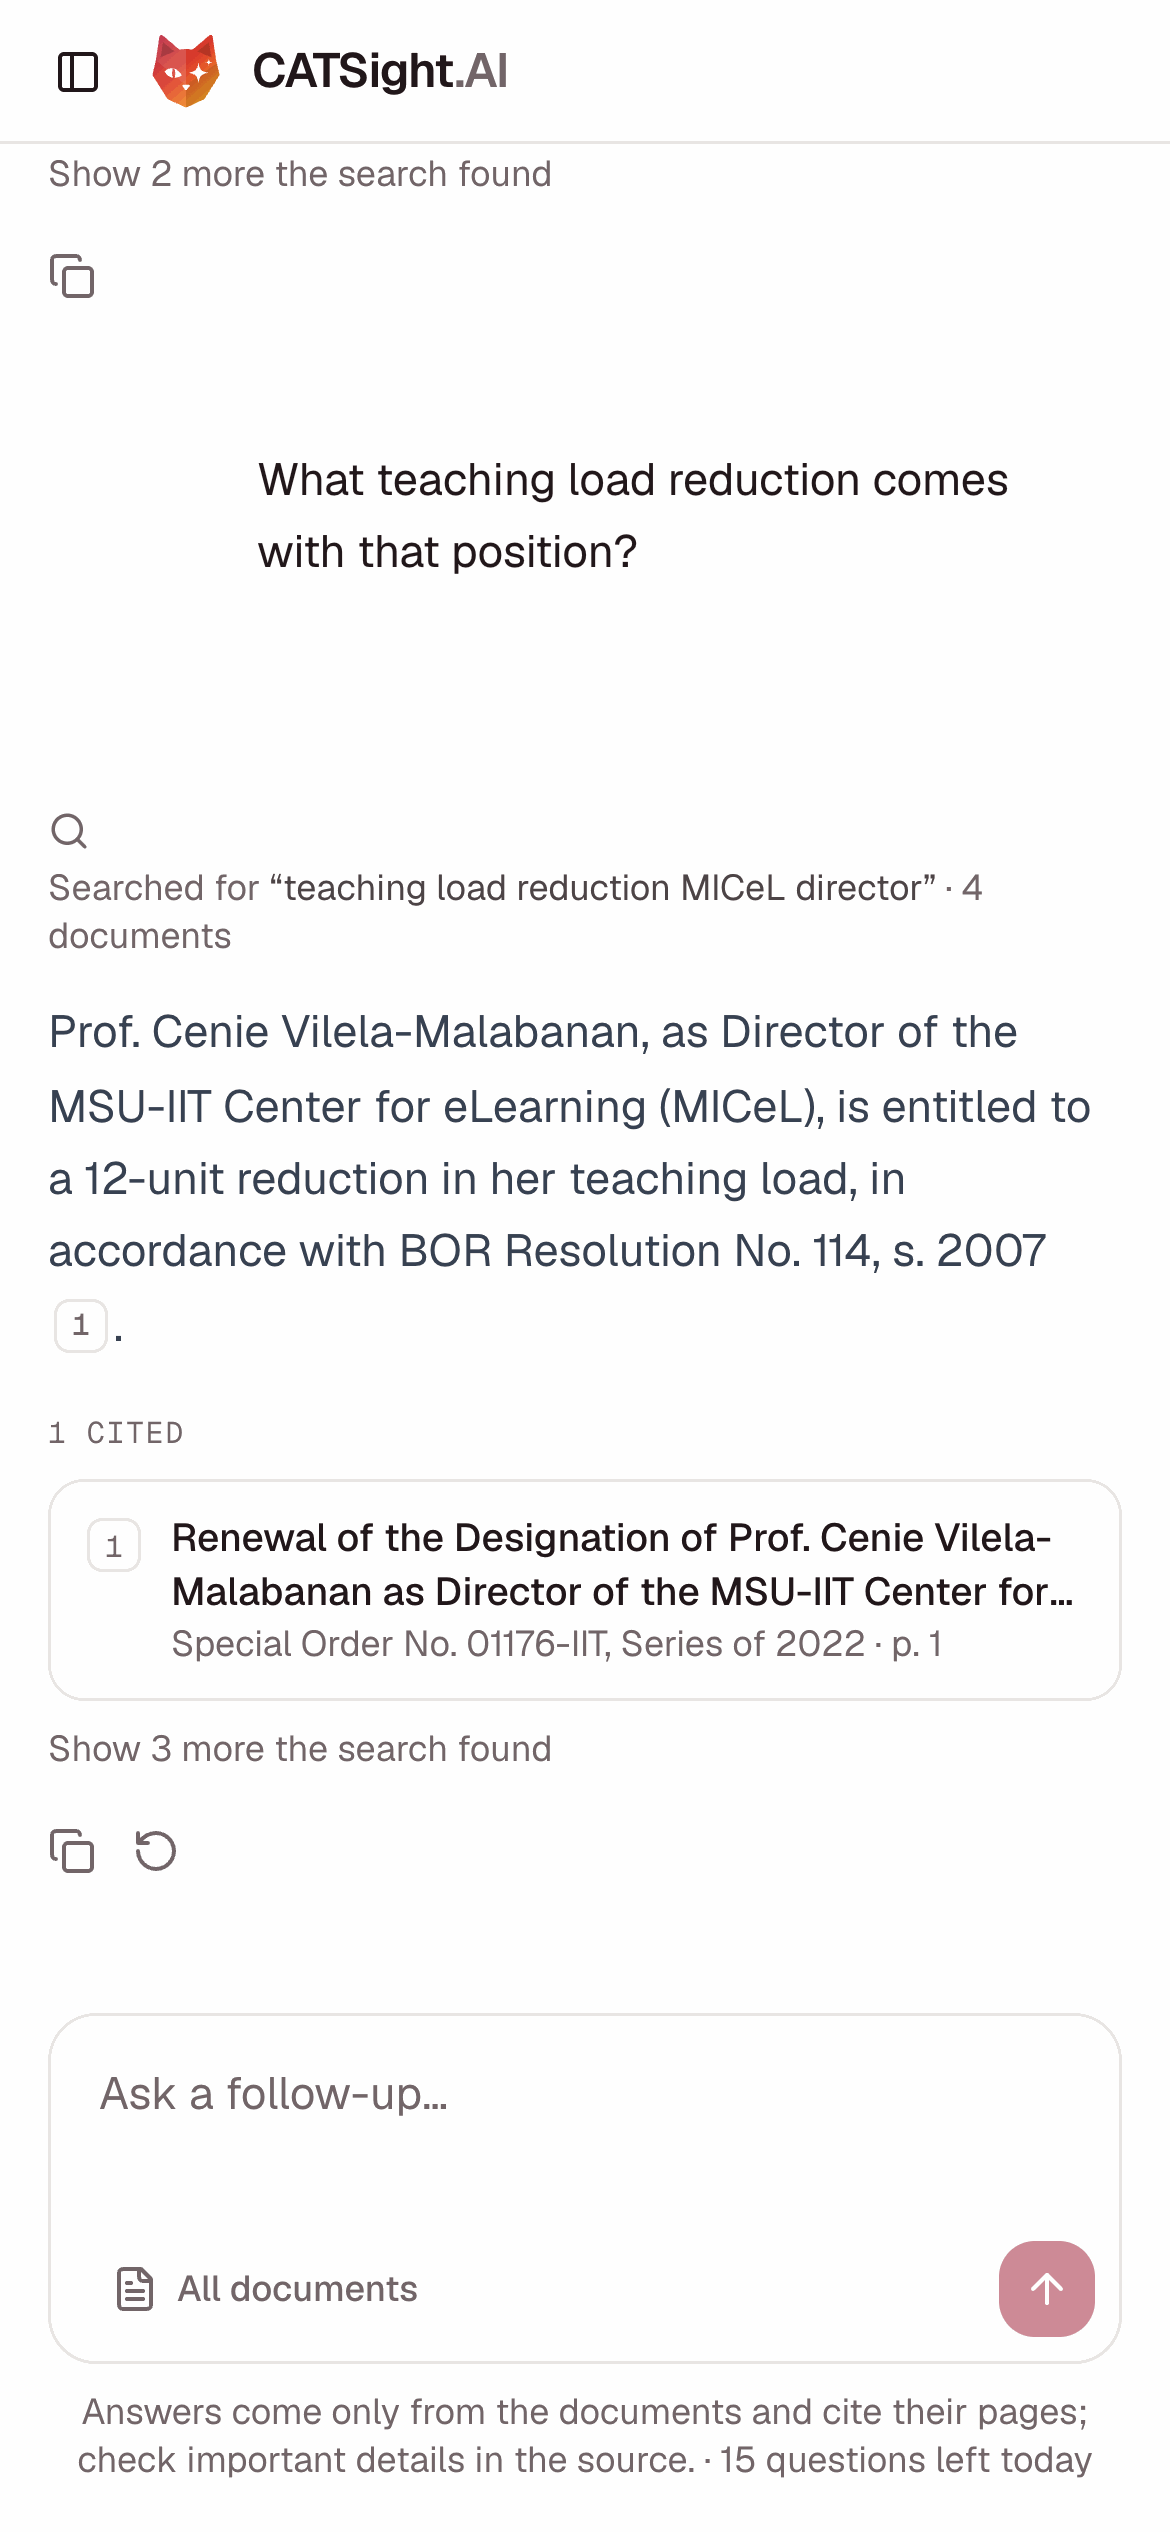
\includegraphics[height=9cm]{screenshots/mobile-chat}}\hspace{1.2cm}%
   \fbox{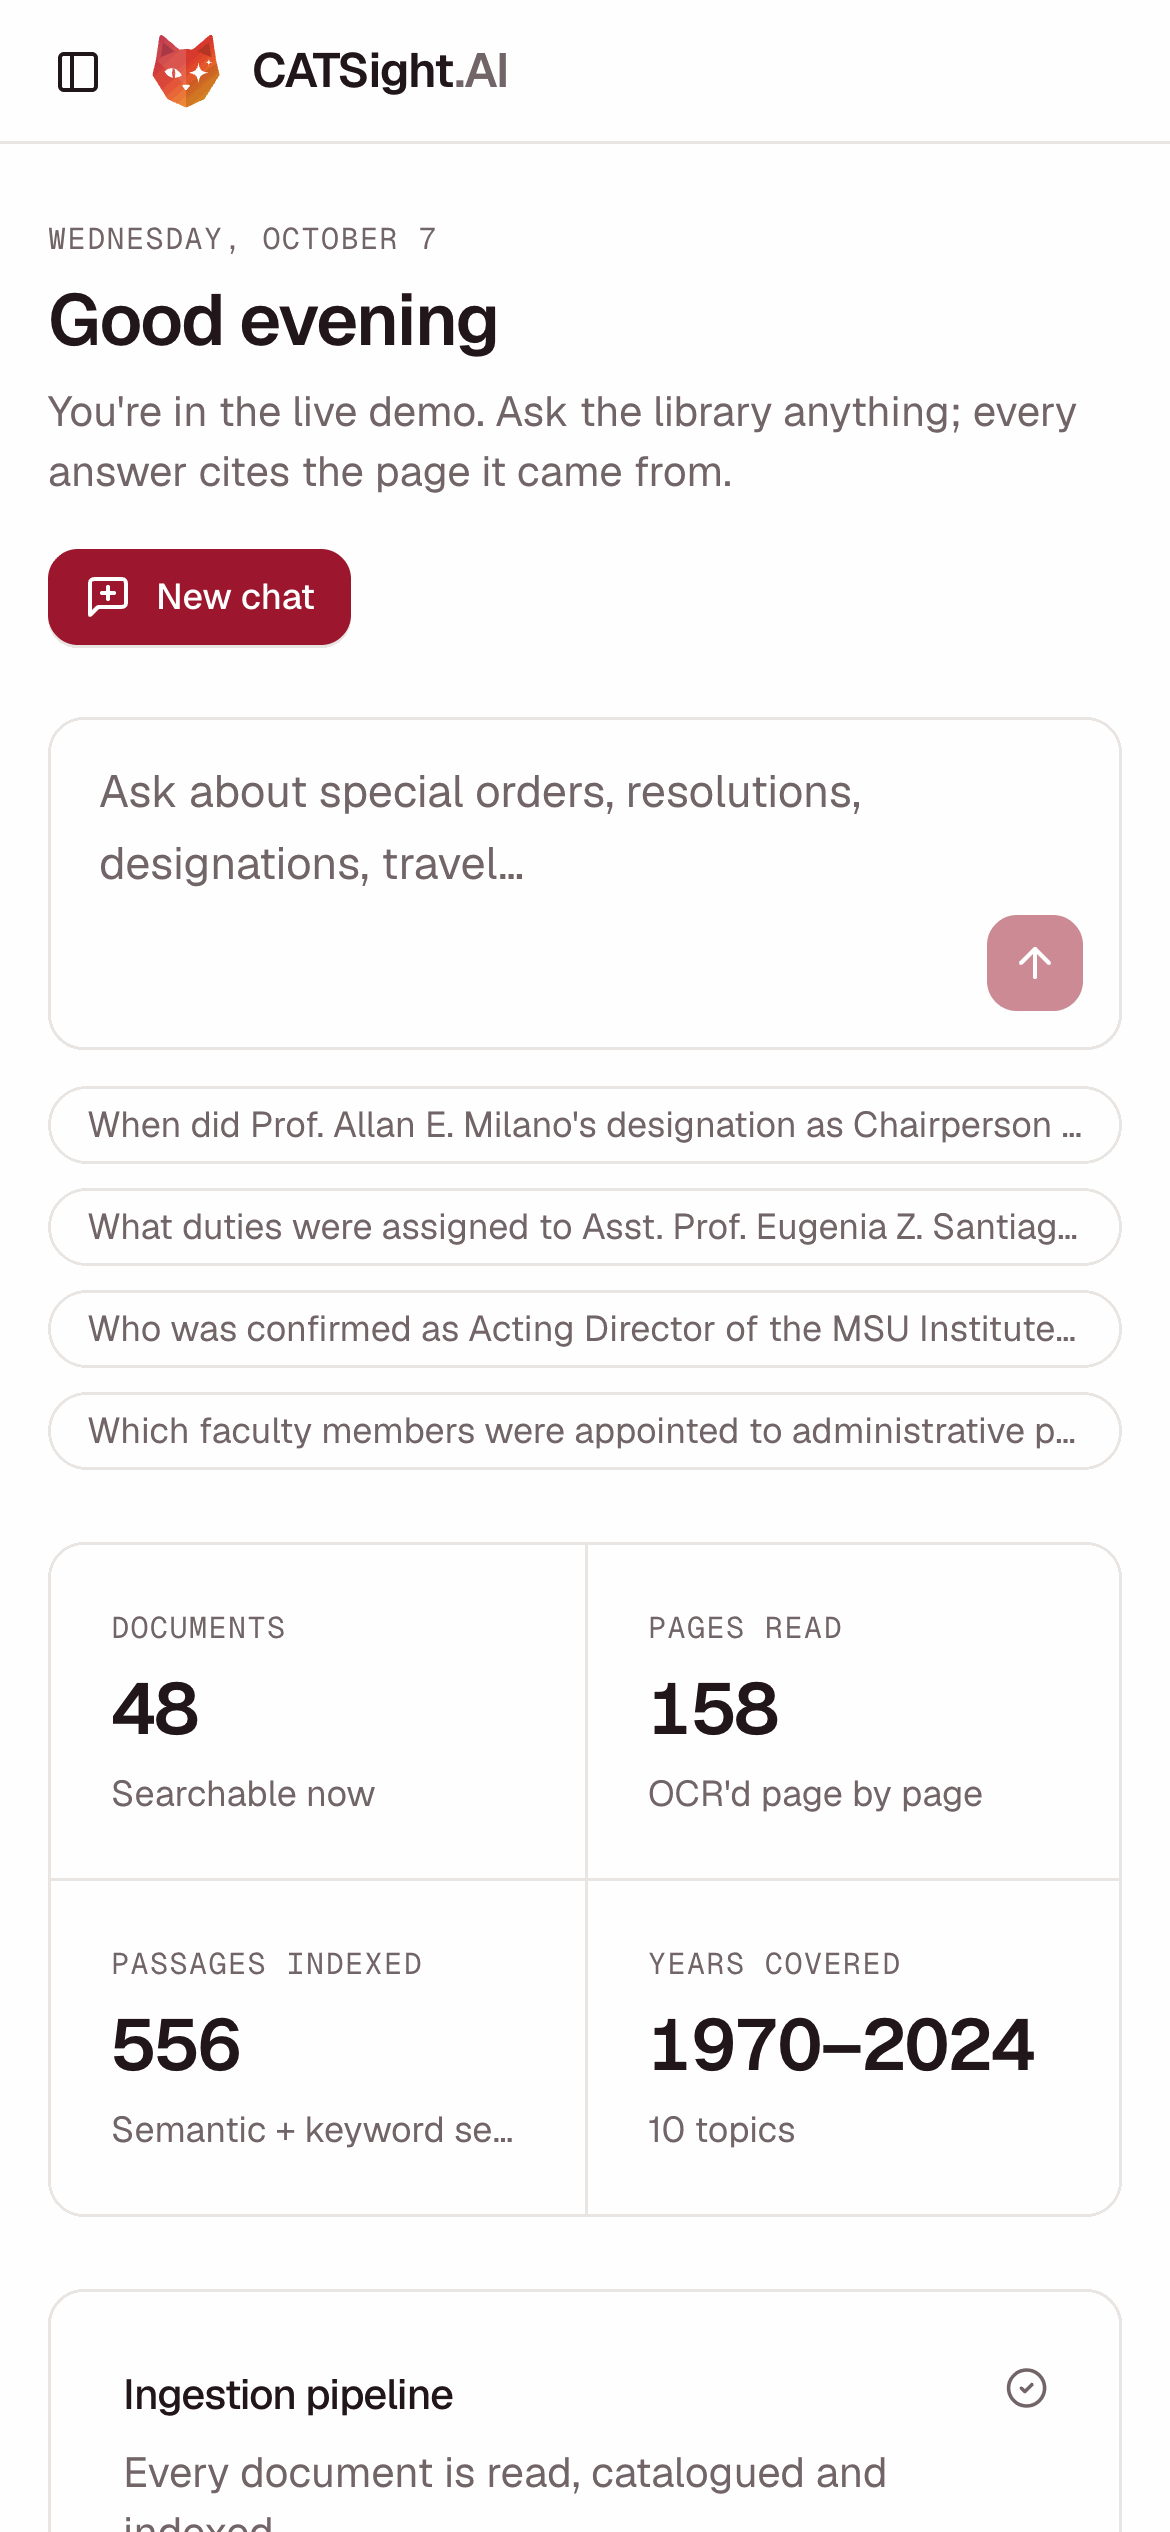
\includegraphics[height=9cm]{screenshots/mobile-dashboard}}}
  \caption{Chat and Dashboard on a Phone}\label{fig:mobile}
\end{figure}

\subsection{Environment and Resources}\label{sec:environment}

Table~\ref{tab:software} lists the software \cs{} is built with. The deployed system runs on a small on-premises server with an integrated GPU, which serves the OCR model; its containers, which cannot use the GPU, are allocated 10 CPU cores and 8~GB of memory. Development and the converter comparison of Section~\ref{sec:converter-comparison} used a laptop with an Apple M4~Pro processor and 24~GB of memory.

\begin{table}[htbp]
  \centering
  \caption{Software Used to Build \cs{}}\label{tab:software}
  \small
  \begin{tabularx}{\linewidth}{@{}>{\raggedright\arraybackslash}p{3.2cm}X@{}}
    \toprule
    \textbf{Layer} & \textbf{Software} \\
    \midrule
    Interface & React 18, TypeScript 5.6, Vite 6, Tailwind CSS 3.4, shadcn/ui, TanStack Query 5, react-pdf 9 (PDF.js) \\
    API & Python 3.11, Django 5.1, Django REST Framework 3.15, gunicorn 23, Server-Sent Events \\
    Document pipeline & Celery 5.5, Redis 7, pypdfium2 4.30, Marker 2.0 with Surya OCR 0.22, llama.cpp (build b11429), PyTorch (CPU) \\
    Retrieval and agent & LangChain 1.x, LangGraph 1.x with a PostgreSQL checkpointer \\
    Database & PostgreSQL 17 with pgvector and full-text search \\
    Models & Surya OCR 2, Qwen3-VL-30B-A3B-Instruct, BGE-M3, Qwen3-Reranker-8B (Table~\ref{tab:models}) through OpenRouter; Ollama for the local configuration \\
    Converters compared & Docling 2.134, MarkItDown 0.1.8 \\
    Deployment & Docker Compose, nginx, an outbound-only HTTPS tunnel \\
    \bottomrule
  \end{tabularx}
\end{table}

\section{Evaluation Procedure}\label{sec:evaluation-procedure}

The system is evaluated with the measures defined in Section~\ref{sec:evaluation-theory}.

\begin{enumerate}
  \item \textbf{Text extraction.} The four converters supported by \cs{} and two vision-model variants are run on a sample of seven documents (26 pages) chosen to cover pure scans, partial text layers, digital files, a watermark, tables, and a typewritten page from 1970. For each document, 8 to 11 facts (reference numbers, names, dates, amounts) were read from the page images, and a converter is credited with a fact when it appears in its output, ignoring case, spacing, punctuation, and leading zeros. Time per page is also recorded.
  \item \textbf{Retrieval accuracy.} A set of test questions, each with the documents that answer it, is run through \cs{}'s search and through the keyword search of IIT Docs; P@5, R@5, and MRR (Equations~\ref{eq:precision-recall} and~\ref{eq:mrr}) are compared. \TODO{Number of test questions and how the relevant documents were judged.}
  \item \textbf{Summary quality.} For a sample of documents, a person writes a reference summary without seeing the generated one; ROUGE-1, ROUGE-2, ROUGE-L, BLEU, and BERTScore (Equations~\ref{eq:rouge-n}--\ref{eq:bertscore}) compare each generated summary with its reference. \TODO{Number of documents and who wrote the references.}
  \item \textbf{Efficiency.} Search time is reported by the server for each search; time to first token and total response time are measured for chat answers; ingestion time is measured per page.
  \item \textbf{Usability.} Participants complete tasks with the existing system and with \cs{} and then answer the SUS questionnaire (Equation~\ref{eq:sus}) for each.
\end{enumerate}
